\documentclass[11pt]{article}
%\usepackage{fullpage,graphicx,algorithm,algorithmic,bm,amsmath,amsthm,amssymb,color,hyperref,cite,natbib}

% if you need to pass options to natbib, use, e.g.:
%\PassOptionsToPackage{numbers}{natbib}
\usepackage{natbib,fullpage}
\usepackage{bm,amsmath,amsthm,amssymb,multicol,algorithmic,algorithm,enumitem}
\usepackage{wrapfig,lipsum}
\usepackage[textwidth=1cm,textsize=footnotesize]{todonotes}

% ready for submission
\usepackage{neurips_2020}

\usepackage[colorlinks=true,
linkcolor=red,
urlcolor=blue,
citecolor=blue]{hyperref}
\usepackage{hyperref}
\usepackage{cleveref}

\setlength{\parskip}{.2cm}


\def\M{\mathcal{M}}
\def\A{\mathcal{A}}
\def\Z{\mathcal{Z}}
\def\S{\mathcal{S}}
\def\D{\mathcal{D}}
\def\R{\mathcal{R}}
\def\P{\mathcal{P}}
\def\K{\mathcal{K}}
\def\E{\mathbb{E}}
\def\F{\mathfrak{F}}
\def\l{\boldsymbol{\ell}}

\newtheorem{Fact}{Fact}
\newtheorem{Lemma}{Lemma}
\newtheorem{Prop}{Proposition}
\newtheorem{Theorem}{Theorem}
\newtheorem{Def}{Definition}
\newtheorem{Corollary}{Corollary}
\newtheorem{Conjecture}{Conjecture}
\newtheorem{Property}{Property}
\newtheorem{Observation}{Observation}
%\theorembodyfont{\rmfamily}
\newtheorem{Exa}{Example}
\newtheorem{assumption}{H\!\!}
\newtheorem{assumptionA}{S\!\!}
\newtheorem{assumptionL}{L\!\!}
\newtheorem{Remark}{Remark}
\newtheorem*{Lemma*}{Lemma}
\newtheorem*{Theorem*}{Theorem}
 \makeatletter
\renewenvironment{proof}[1][\proofname]{%
   \par\pushQED{\qed}\normalfont%
   \topsep6\p@\@plus6\p@\relax
   \trivlist\item[\hskip\labelsep\bfseries#1]%
   \ignorespaces
}{%
   \popQED\endtrivlist\@endpefalse
}
\makeatother

%%%%%%%%%%% Stuffs for Tikz %%%%%%%%%%%%%%%%%%
\usepackage{pgfplots}
\usepackage{xargs}
\usepackage{stmaryrd}
\usetikzlibrary{arrows,shapes,calc,tikzmark,backgrounds,matrix,decorations.markings}
\usepgfplotslibrary{fillbetween}

\pgfplotsset{compat=1.3}

\usepackage{relsize}
\tikzset{fontscale/.style = {font=\relsize{#1}}
    }

\definecolor{lavander}{cmyk}{0,0.48,0,0}
\definecolor{violet}{cmyk}{0.79,0.88,0,0}
\definecolor{burntorange}{cmyk}{0,0.52,1,0}

\def\lav{lavander!90}
\def\oran{orange!30}

\definecolor{asuorange}{rgb}{1,0.699,0.0625}
\definecolor{asured}{rgb}{0.598,0,0.199}
\definecolor{asuborder}{rgb}{0.953,0.484,0}
\definecolor{asugrey}{rgb}{0.309,0.332,0.340}
\definecolor{asublue}{rgb}{0,0.555,0.836}
\definecolor{asugold}{rgb}{1,0.777,0.008}

%%%%%%%%%%%%%%%%%%%%%%%%%%%%%%%%%%%%%


\usepackage{shortcuts_OPT}

%\renewcommand{\textwidth}{5.5in}

% Here's the definition of Sb, stolen from amstex
    \makeatletter
    \def\multilimits@{\bgroup
  \Let@
  \restore@math@cr
  \default@tag
 \baselineskip\fontdimen10 \scriptfont\tw@
 \advance\baselineskip\fontdimen12 \scriptfont\tw@
 \lineskip\thr@@\fontdimen8 \scriptfont\thr@@
 \lineskiplimit\lineskip
 \vbox\bgroup\ialign\bgroup\hfil$\m@th\scriptstyle{##}$\hfil\crcr}
    \def\Sb{_\multilimits@}
    \def\endSb{\crcr\egroup\egroup\egroup}
\makeatother

\newtheoremstyle{k}         %name
    {\baselineskip}{2\topsep}      %space above and below
    {\rm}                   %Body font
    {0pt}{\bfseries}  %Heading indent and font
    {}                      %after heading
    { }                      %head after space
    {\thmname{#1}\thmnumber{#2}.}

\theoremstyle{k}
\newtheorem{q}{Q}
\parindent=0pt

%\newcommand{\eric}[1]{\todo[color=red!20]{{\bf EM:} #1}}
%\newcommand{\erici}[1]{\todo[color=red!20,inline]{{\bf EM:} #1}}
%\newcommand{\belhal}[1]{\todo[color=green!20]{{\bf BK:} #1}}
%\newcommand{\belhali}[1]{\todo[color=green!20,inline]{{\bf BK:} #1}}
%\newcommand{\toco}[1]{\todo[color=yellow!20]{{\bf To:} #1}}



\makeatletter
\DeclareRobustCommand*\cal{\@fontswitch\relax\mathcal}
\makeatother

\begin{document}
\title{OPT-AMSGrad: An Optimistic Acceleration of AMSGrad for Nonconvex Optimization}
%\author{}
\date{\today}

\maketitle


\begin{abstract}
We consider a new variant of AMSGrad. 
AMSGrad \cite{RKK18} is a popular adaptive gradient based optimization algorithm that is widely used in training deep neural networks. 
The new variant assumes that mini-batch gradients in consecutive iterations have some underlying structure, which makes the gradients sequentially predictable. 
By exploiting the predictability and some ideas from Optimistic Online Learning, the proposed algorithm can accelerate the convergence, increase sample efficiency and also enjoys a tighter non-asymptotic bound under some conditions. 
We conduct experiments on several deep learning models, which show that by improving sample efficiency, the proposed method achieves a convergence speedup in practice.
\end{abstract}

\section{Introduction}

Nowadays deep learning has been very successful in several applications, from 
robotics (e.g. \cite{LFDA17}), 
computer vision (e.g. \cite{Rnet16,goodfellow2014generative}),
reinforcement learning (e.g. \cite{Atari13}),
to 
natural language processing (e.g. \cite{GMH13}).
A common goal in these applications is learning quickly.
It becomes a desired goal 
due to the presence of big data and/or the use of large neural nets.
To accelerate the process, there are number of algorithms proposed in recent years, such as 
\textsc{AMSGrad} \cite{RKK18}, 
\textsc{ADAM} \cite{KB15}, \textsc{RMSPROP} \cite{TH12}, \textsc{ADADELTA} \cite{Z12}, and \textsc{NADAM} \cite{D16}, etc.

All the prevalent algorithms for training deep nets mentioned above combine two ideas: the idea of adaptivity from \textsc{AdaGrad} \cite{DHS11,MS10} and the idea of momentum from \textsc{Nesterov's  Method} \cite{N04} or \textsc{Heavy ball} method \cite{P64}.
\textsc{AdaGrad} is an online learning algorithm that works well compared to the standard online gradient descent when the gradient is sparse.
Its update has a notable feature: the learning rate is different for each dimension, depending on the magnitude of gradient in each dimension, which might help in exploiting the geometry of data and leading to a better update. 
On the other hand,
\textsc{Nesterov's Method} or \textsc{Heavy ball} Method \cite{P64} is an accelerated optimization algorithm whose update not only depends on the current iterate and current gradient but also depends on the past gradients (i.e. momentum). State-of-the-art algorithms like \textsc{AMSGrad} \cite{RKK18} and \textsc{ADAM} \cite{KB15} leverage this ideas to accelerate the training process of neural nets.

In this paper, we propose an algorithm that goes further than the hybrid of the adaptivity and momentum approach. Our algorithm is inspired by \textsc{Optimistic Online learning} \cite{CJ12,RS13,SALS15,ALLW18}, which assumes that a good guess of the loss function in each round of online learning is available, and plays an action by exploiting the guess. 
By exploiting the guess, algorithms in 
\textsc{Optimistic Online learning}
can enjoy smaller regret than the ones without exploiting the guess.
We combine the \textsc{Optimistic Online learning} idea with the adaptivity and the momentum ideas to design a new algorithm --- \textsc{Optimistic-AMSGrad}. To the best of our knowledge, this is the first work exploring towards this direction. The proposed algorithm
not only adapts to the informative dimensions, exhibits momentum, but also exploits a good guess of the next gradient to facilitate acceleration. Besides theoretical analysis of \textsc{Optimistic-AMSGrad}, we also conduct experiments and show that the proposed algorithm not only accelerates convergence of loss function, but also leads to better generalization performance in some cases.

%\vspace{-0.1in}
\section{Preliminaries}
%\vspace{-0.1in}
We begin by providing some background in online learning, as we use some tools from it to 
design and analyze the proposed algorithm.
We follow the notations in related adaptive optimization papers \cite{KB15,RKK18}. For any vector $u$, $v \in \mathbb R^{d}$,  $u/v$ represents element-wise division,
$u^{2}$ represents element-wise square, $\sqrt{u}$ represents element-wise square-root.
We denote $g_{1:T}[i]$ as the sum of the $i_{th}$ element of $T$ vectors $g_{1}, g_{2},
\dots, g_{T} \in \mathbb R^{d}$.

\subsection{Optimistic Online learning}
%\vspace{-0.05in}
The standard setup of \textsc{Online learning} is that,
in each round $t$, an online learner selects an action $w_{t} \in \K \subseteq \mathbb R^{d}$,
then the learner observes $\ell_{t}(\cdot)$ and suffers loss $\ell_{t}(w_t)$
after the learner commits the action.
The goal of the learner is minimizing the regret,
$$\text{Regret}_{T}( \{ w_t \} ):= \sum_{t=1}^T \ell_{t}(w_t) - \sum_{t=1}^T \ell_{t}(w^*),$$
which is the cumulative loss of the learner minus the cumulative loss of
some benchmark $w^{*} \in \K$.

%In recent years, there are some works for  
%\textsc{Optimistic Online learning} 
The idea of \textsc{Optimistic Online learning} (e.g. \cite{CJ12,RS13,SALS15,ALLW18})
is as follows.
Suppose that, in each round $t$, the learner has a good guess $m_t(\cdot)$ of the loss function $\ell_t(\cdot)$ before playing an action $w_t$. 
Then, the learner should exploit the guess $m_t(\cdot)$ to choose an action $w_t$ since $m_t(\cdot)$ is close to the true loss function $\ell_t(\cdot)$.
\footnote{Imagine that if the learner would had been known $\ell_t(\cdot)$ before committing its action, then it would exploit the knowledge to determine its action and consequently minimizes the regret.} For example, \cite{SALS15} proposes an optimistic-variant of \textsc{Follow-the-Regularized-Leader} (\textsc{FTRL}).
%The update rule of (non-optimistic) 
\textsc{FTRL} (see e.g. \cite{H14}) is an online learning algorithm whose update is
\begin{equation} \label{optFTRL}
\textstyle w_t  = \arg \min_{w \in \K} \langle w , L_{t-1} \rangle + \frac{1}{\eta} R(w),
\end{equation}
where $\eta$ is a parameter, $R(\cdot)$ is a $1$-strongly convex function with respect to a norm ($\| \cdot \|$) on the constraint set $\K$, and
$L_{t-1}:= \sum_{s=1}^{t-1} g_s$ is the cumulative sum of gradient vectors of 
the loss functions (i.e. $g_s := \nabla \ell_s(w_s)$ ) up to but not including $t$.
FTRL has regret at most $O(\sqrt{\sum_{t=1}^T \| g_t \|_*})$.
On the other hand, \textsc{Optimistic-FTRL} \cite{SALS15} has update  
\begin{equation} \label{optFTRL}
\textstyle w_t  = \arg \min_{w \in \K} \langle w , L_{t-1} + m_t \rangle + \frac{1}{\eta} R(w),
\end{equation}
where 
$m_{t}$ is the learner's guess of the gradient vector $g_{t}:=\nabla \ell_t(w_t)$.
Under the assumption that loss functions are convex,
the regret of \textsc{Optimistic-FTRL} is at most
%\begin{equation}
$O(\sqrt{\sum_{t=1}^T \| g_t - m_t \|_*  } )$,
%\end{equation}
which can be much smaller than the regret of \textsc{FTRL} if $m_{t}$ is close to $g_{t}$.
Consequently, \textsc{Optimistic-FTRL} can achieve better performance than $\textsc{FTRL}$.
%The concern is that how to get good $m_t$. 
On the other hand, if $m_t$ is far from $g_t$, then 
the regret of \textsc{Optimistic-FTRL} would be only a constant factor worse than that of its counterpart \textsc{FTRL}. 
In Section~\ref{sec:predict_m}, we will provide a way to get $m_t$. Now we just want to emphasize the importance of leveraging a good guess $m_t$ for updating $w_t$ in order to get a fast convergence rate (or equivalently, small regret). We will have a similar argument when we compare \textsc{Optimistic-AMSGrad} and \textsc{AMSGrad}.
%We are also aware of the works of \cite{CJ12,RS13,SALS15}), which show that Optimistic-algorithms can accelerate the convergence of some zero-sum games.

\subsection{Adaptive optimization methods}



Recently, adaptive optimization has been popular in various deep learning applications due to their superior empirical performance. \textsc{Adam} \cite{KB15} is a very popular adaptive algorithm for training deep nets.
It combines the momentum idea \cite{P64} with the idea of \textsc{AdaGrad} \cite{DHS11},
which has different learning rates for different dimensions, adaptive to the learning process. More specifically, the learning rate of \textsc{AdaGrad} in iteration $t$ for a dimension $j$ is proportional to the inverse of $\sqrt{ \Sigma_{s=1}^t g_s[j]^2 }$,
where $g_s[j]$ is the $j$-th element of the gradient vector $g_s$ 
at time $s$.
This adaptive learning rate might help for accelerating the convergence when the gradient vector is sparse \cite{DHS11}. However,
when applying \textsc{AdaGrad} to train deep nets,
it is observed that the learning rate might decay too fast \cite{KB15}.
Therefore, \cite{KB15} proposes using a moving average of gradients 
divided by the square root of the second moment of the moving average (element-wise fashion), for updating the model parameter $w$ (i.e. line 5,6 and line 8 of Algorithm~\ref{alg:amsgrad}).
Yet, \textsc{Adam} \cite{KB15} fails at some online convex optimization problems. \textsc{AMSGrad}~\cite{RKK18} fixes the issue. 
The algorithm of \textsc{AMSGrad} is shown in Algorithm~\ref{alg:amsgrad}.
The difference between \textsc{Adam} and 
\textsc{AMSGrad} lies on line 7 of Algorithm~\ref{alg:amsgrad}.
\textsc{Adam} does not have the max operation on line 7 (i.e. $\hat{v}_t = v_t$ for \textsc{Adam}) while
\cite{RKK18} adds the operation to guarantee a non-increasing learning rate,
$\frac{\eta_t }{ \sqrt{\hat{v}}_t }$,
which helps for the convergence (i.e. average regret $\frac{\text{Regret}_T}{T} \rightarrow 0$).
For the hyper-parameters of \textsc{AMSGrad}, it is suggested in~\cite{RKK18} that $\beta_1=0.9$ and $\beta_2=0.99$.


\begin{algorithm}[H]
\begin{algorithmic}[1]
\small
\caption{\textsc{AMSGrad} \cite{RKK18}} \label{alg:amsgrad}
\STATE Required: parameter $\beta_1$, $\beta_2$, and $\eta_t$. 
\STATE Init: $w_{1} \in \K \subseteq \mathbb R^d $ and $v_{0} = \epsilon 1 \in \mathbb R^{d}$.
\FOR{$t=1$ to $T$}
\STATE Get mini-batch stochastic gradient vector $g_t$ at $w_t$.
\STATE $\theta_t = \beta_1 \theta_{t-1} + (1 - \beta_1) g_t$.
\STATE $v_t = \beta_2 v_{t-1} + (1 - \beta_2) g_t^2$. 
\STATE $\hat{v}_t = \max( \hat{v}_{t-1} , v_t )$. 
\STATE $w_{t+1} = w_t - \eta_t \frac{\theta_t}{ \sqrt{\hat{v}}_t }$.
\text{ (element-wise division)}
\ENDFOR
\end{algorithmic}
\end{algorithm}


%\vspace{-0.1in}
\section{\textsc{Optimistic-AMSGrad}}
%\vspace{-0.1in}
%{\color{blue} Maybe we can just call it \textsc{Optimistic-amsgrad}? }
We propose a new optimization algorithm,
\textsc{Optimistic-AMSGrad}, shown in Algorithm~\ref{alg:optamsgrad}. It combines the idea of adaptive optimization with optimistic learning. In each iteration, the learner computes a gradient vector $g_{t}:= \nabla \ell_t( w_t)$ at $w_{t}$ (line 4), then it maintains an exponential moving average of $\theta_{t} \in \mathbb R^{d}$ (line 5) and $v_{t} \in \mathbb R^{d}$ (line 6), which is followed by
the max operation to get $\hat{v}_{t} \in \mathbb R^{d}$ (line 7).
The learner also updates an auxiliary variable $w_{t+\frac{1}{2}} \in \K$ (line 8). It uses the auxiliary variable (hidden model) to update and commit $w_{t+1}$ (line 9), which exploits the guess $m_{t+1}$ of $g_{t+1}$ to get $w_{t+1}$.
As the learner's action set is $\K \subseteq \mathbb R^{d}$, we adopt the notation $\Pi_{\K}[\cdot]$ for the projection to $\K$ if needed. The scheme of \textsc{AMSGrad} is summarized in Figure \ref{scheme}.


%\begin{tabular}{cc}
%\raisebox{-.1cm}{\begin{minipage}{.5\textwidth}
%\begin{algorithm}[H]
%\caption{OPTIMISTIC-AMSGRAD}\label{alg:opt-ams}
%  \begin{algorithmic}[1]
%  \STATE \textbf{Input:} Parameters $\beta_{1}, \beta_{2}, \epsilon, \eta_{k}$
%  \STATE \textbf{Init.:} $w_{1}=w_{-1 / 2} \in \mathcal{K} \subseteq \mathbb{R}^{d} \text { and } v_{0}=\epsilon \mathbf{1} \in \mathbb{R}^{d}$
%  \FOR {$k=1,2,\dots, K$}
%  \STATE Get mini-batch stochastic gradient $g_{k}$ at $w_{k}$
%   \STATE $\theta_{k}=\beta_{1} \theta_{k-1}+\left(1-\beta_{1}\right) g_{k}$
%   \STATE $v_{k}=\beta_{2} v_{k-1}+\left(1-\beta_{2}\right) g_{k}^{2}$
%   \STATE $ \hat{v}_{k}=\max \left(\hat{v}_{k-1}, v_{k}\right)$
%   \STATE $ w_{k+\frac{1}{2}}=\Pi_{\mathcal{K}}\left[w_k-\eta_{k} \frac{\theta_{k}}{\sqrt{\hat{v}_{k}}}\right]$
%   \STATE $ w_{k+1}=\Pi_{\mathcal{K}}\left[w_{k+\frac{1}{2}}-\eta_{k} \frac{h_{k+1}}{\sqrt{v}_{k}}\right]$
%where $ \quad h_{k+1}:=\beta_{1} \theta_{k-1} + (1-\beta_{1}) m_{k+1}$
%      \STATE $ \quad\quad \text{and} \quad m_{k+1}$ is a guess of $g_{k+1}$
%\ENDFOR
%\STATE \textbf{Return}: $w_{K+1}$.
%  \end{algorithmic}
%\end{algorithm}\vspace{.1cm}
%\end{minipage}} &
%\begin{minipage}{.5\textwidth}
%\begin{figure}[H]
%    % \centering
%    \hspace{-0.15in}
%    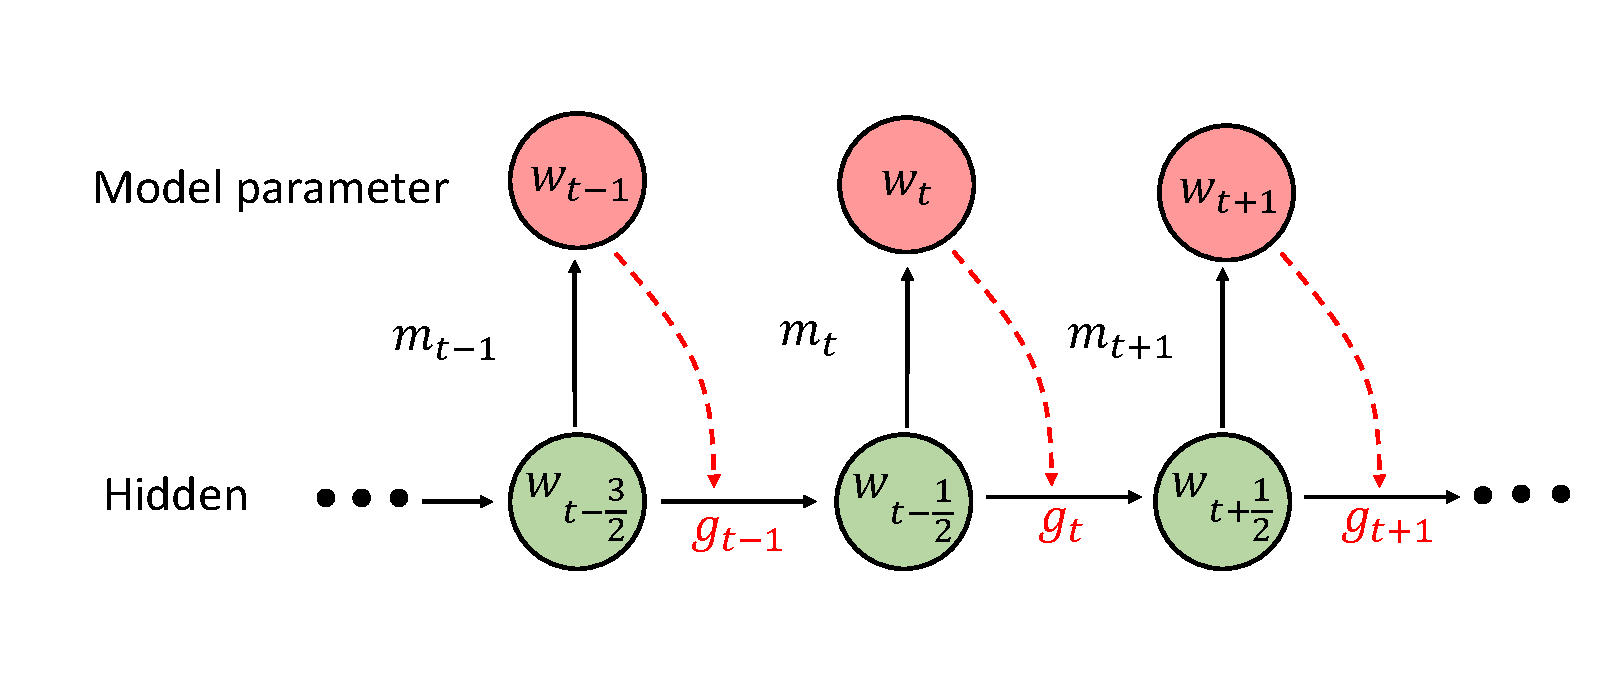
\includegraphics[width=2.6in]{plot.pdf}
%    \caption{Scheme of \textsc{OPTIMISTIC-AMSGRAD}.}
%     \label{scheme}
%\end{figure}
%
%\end{minipage}
%\end{tabular}

\begin{algorithm}[H]
\caption{OPTIMISTIC-AMSGRAD}\label{alg:optamsgrad}
  \begin{algorithmic}[1]
  \STATE \textbf{Input:} Parameters $\beta_{1}, \beta_{2}, \epsilon, \eta_{k}$
  \STATE \textbf{Init.:} $w_{1}=w_{-1 / 2} \in \mathcal{K} \subseteq \mathbb{R}^{d} \text { and } v_{0}=\epsilon \mathbf{1} \in \mathbb{R}^{d}$
  \FOR {$k=1,2,\dots, K$}
  \STATE Get mini-batch stochastic gradient $g_{k}$ at $w_{k}$
   \STATE $\theta_{k}=\beta_{1} \theta_{k-1}+\left(1-\beta_{1}\right) g_{k}$
   \STATE $v_{k}=\beta_{2} v_{k-1}+\left(1-\beta_{2}\right) g_{k}^{2}$
   \STATE $ \hat{v}_{k}=\max \left(\hat{v}_{k-1}, v_{k}\right)$
   \STATE $ w_{k+\frac{1}{2}}=\Pi_{\mathcal{K}}\left[w_k-\eta_{k} \frac{\theta_{k}}{\sqrt{\hat{v}_{k}}}\right]$
   \STATE $ w_{k+1}=\Pi_{\mathcal{K}}\left[w_{k+\frac{1}{2}}-\eta_{k} \frac{h_{k+1}}{\sqrt{v}_{k}}\right]$
where $ \quad h_{k+1}:=\beta_{1} \theta_{k-1} + (1-\beta_{1}) m_{k+1}$
      \STATE $ \quad\quad \text{and} \quad m_{k+1}$ is a guess of $g_{k+1}$
\ENDFOR
\STATE \textbf{Return}: $w_{K+1}$.
  \end{algorithmic}
\end{algorithm}\vspace{.1cm}

\begin{figure}[H]
    % \centering
    \hspace{-0.15in}
    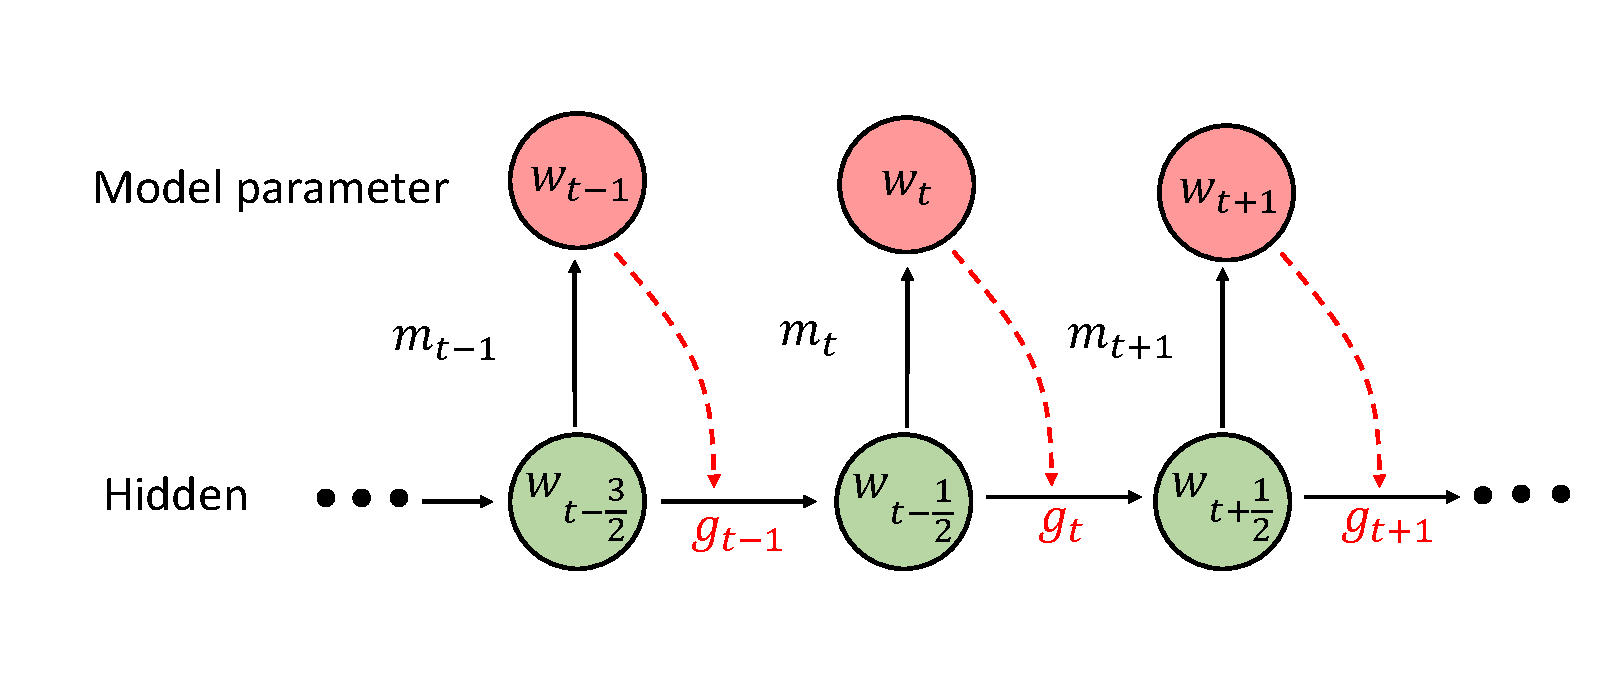
\includegraphics[width=4.6in]{plot.pdf}
    \caption{Scheme of \textsc{OPTIMISTIC-AMSGRAD}.}
     \label{scheme}
\end{figure}


We see that the proposed \textsc{Optimistic-AMSGrad} inherits three properties:
%\vspace{-0.1in}
\begin{itemize}
\item Adaptive learning rate of each dimension as \textsc{AdaGrad} \cite{DHS11}. (line 6, line 8 and line 9)
\item Exponential moving average of the past gradients as \textsc{Nesterov's method} \cite{N04} and the \textsc{Heavy-Ball} method \cite{P64}. (line 5)
\item Optimistic update that exploits a good guess of the next gradient vector
as optimistic online learning algorithms \cite{CJ12,RS13,SALS15}. (line 9)
\end{itemize}
%\vspace{-0.1in}

The first property helps for acceleration when the gradient has a sparse structure.
The second one is from the well-recognized idea of momentum which can also help for acceleration. The last one, perhaps less known outside the \textsc{Online learning} community, can actually lead to acceleration when the prediction of the next gradient is good. This property will be elaborated in the following subsection in which we provide the theoretical analysis of \textsc{Optimistic-AMSGrad}.


Observe that the proposed algorithm does not reduce to \textsc{AMSGrad} when $m_{t}=0$.
Furthermore, if $\K = \mathbb R^{d}$ (unconstrained case), one might want to combine line 8 and line 9 and get a single line as 
\beq\label{eq:finalupdate}
w_{k+1}=w_{k}-\eta_{k} \frac{\theta_{k}}{\sqrt{\hat{v}_{k}}}-\eta_{k} \frac{h_{k+1}}{\sqrt{v}_{k}}
\eeq
Yet, based on this expression, we see that $w_{t+1}$ is updated from $w_{t-\frac{1}{2}}$ instead of $w_t$. Therefore, while \textsc{Optimistic-AMSGrad} looks like just doing an additional update compared to \textsc{AMSGrad}, the difference of the updates is subtle.
In the following analysis, we show that the interleaving actually leads to some cancellation in the regret bound.



%\vspace{-0.15in}


\subsection{Theoretical analysis}
\textcolor{red}{TO COMPLETE}

In this section, we provide regret analysis of the proposed method and show that it may improve the bound of vanilla \textsc{AMSGrad} with good guess of gradient.

\textbf{Notations.}\hspace{0.1in}To begin with, let us introduce some notations first.
We denote the Mahalanobis norm $\|\cdot\|_H := \sqrt{ \langle \cdot, H \cdot \rangle }$ for some PSD matrix $H$.
We let $\psi_t(x) := \langle x, \text{diag}\{\hat{v}_t\}^{1/2} x \rangle$ for a PSD matrix $H_t^{1/2}:= \text{diag}\{\hat{v}_t\}^{1/2}$, 
%Denote the PSD matrix $H_t := \text{diag}\{\hat{v}_t\}$, 
where $\text{diag}\{\hat{v}_t\}$ represents the diagonal matrix whose $i_{th}$ diagonal element is $\hat{v}_t[i]$ in Algorithm~\ref{alg:optamsgrad}.
We define its corresponding Mahalanobis norm $\| \cdot \|_{\psi_t}:= 
\sqrt{ \langle \cdot, \text{diag}\{\hat{v}_t\}^{1/2} \cdot \rangle }$,
where we abuse the notation $\psi_t$ to represent the PSD matrix $H_t^{1/2}:=\text{diag}\{\hat{v}_t\}^{1/2}$.
Consequently,
$\psi_t(\cdot)$ is 1-strongly convex with respect to the norm $\| \cdot \|_{\psi_t}:= 
\sqrt{ \langle \cdot, \text{diag}\{\hat{v}_t\}^{1/2} \cdot \rangle }$.
Namely, $\psi_t(\cdot)$ satisfies
$\psi_t(u) \geq \psi_t(v) + \langle \psi_t(v), u - v \rangle + \frac{1}{2} \| u - v\|^2_{\psi_t}$
for any point $u,v$.
A consequence of 1-strongly convexity of $\psi_t(\cdot)$ is that
$B_{\psi_t}(u,v) \geq \frac{1}{2} \| u - v \|^2_{\psi_t}$,
where the Bregman divergence $B_{\psi_t}(u,v)$ is defined as 
$B_{\psi_t}(u,v) := \psi_t(u)
- \psi_t(v) - \langle \psi_t(v), u - v \rangle
$ with $\psi_t(\cdot)$ as the distance generating function.
We can also define the corresponding dual norm $\| \cdot \|_{\psi_t^*}:= \sqrt{ \langle \cdot, \text{diag}\{\hat{v}_t\}^{-1/2} \cdot \rangle }$.

\textbf{Non-asymptotic analysis.}\hspace{0.1in}We establish in this section a finite-time upper bound of the expected squared norm of the gradient of the objective function we are optimizing.
The objective function for most deep learning task reads as follows:
\begin{equation}\label{eq:minproblem}
\min \limits_{w \in \Theta} f(w) \eqdef  \frac{1}{n} \sum_{i=1}^n f(w, \xi_i)
\end{equation}
where $(\xi_i, i \in [1,n])$ is the vector of $n$ input data.

\subsection{Comparison to some related methods} \label{app:related}

\textbf{Comparison to nonconvex optimization works.}\hspace{0.1in}Recently, \cite{ZRSKK18,CLSH19,WWB18,ZTYCG18,ZS18,LO18} provide some theoretical analysis 
of \textsc{Adam}-type algorithms when applying them to smooth nonconvex optimization problems.
For example, \cite{CLSH19} provides a bound,
which is $\min_{t \in [T]} \mathbb{E}[\| \nabla f(w_t) \|^2 ] = O(\log T / \sqrt{T}) $.
Yet, this data independent bound does not show any advantage over standard stochastic gradient descent. Similar concerns appear in other papers.

To get some adaptive data dependent bound (e.g. bounds like (\ref{bc}) or (\ref{boundAMS})
that are in terms of the gradient norms observed along the trajectory) when applying 
\textsc{Optimistic-AMSGrad} to nonconvex optimization,
one can follow the approach of \cite{Princeton18} or \cite{CYYZC19}.
They provide ways to convert algorithms with adaptive data dependent regret bound
for convex loss functions (e.g. \textsc{AdaGrad}) to the ones that can find an approximate stationary point of non-convex loss functions. 
Their approaches are modular so that simply using \textsc{Optimistic-AMSGrad}
as the base algorithm in their methods will immediately lead to a variant of \textsc{Optimistic-AMSGrad} that enjoys some guarantee on nonconvex optimization.
The variant can outperform the ones instantiated by other \textsc{Adam}-type algorithms when
the gradient prediction $m_t$ is close to $g_t$.
The details are omitted since this is a straightforward application.

\textbf{Comparison to AO-FTRL \cite{MY16}.}\hspace{0.1in}In \cite{MY16}, the authors propose AO-FTRL, which has the update of 
the form $w_{t+1} = \arg\min_{{w \in \K}} ( \sum_{s=1}^t g_s )^{\top}  w + m_{t+1}^\top w + r_{0:t}(w) $, where $r_{0:t}(\cdot)$ is a 1-strongly convex loss function with respect to some norm $\| \cdot\|_{(t)}$ that may be different for different iteration $t$. 
Data dependent regret bound was provided in the paper, which is $r_{{0:T}}(w^*) + \sum_{t=1}^T \| g_t - m_t \|_{(t)^*}$ for any benchmark $w^{*} \in \K$. We see that if
one selects $r_{0:t}(w) := \langle w, \text{diag}\{\hat{v}_t\}^{1/2} w \rangle$ 
and $\| \cdot \|_{(t)}:= 
\sqrt{ \langle \cdot, \text{diag}\{\hat{v}_t\}^{1/2} \cdot \rangle }$, then the update might be viewed as an optimistic variant of $\textsc{AdaGrad}$. However, no experiments was provided in \cite{MY16}. 


\textbf{Comparison to \textsc{Optimistic-Adam}~\cite{DISZ18}.}\hspace{0.1in}We are aware that \cite{DISZ18} proposed one version of optimistic algorithm for ADAM, which
is called \textsc{Optimistic-Adam} in their paper. A slightly modified version is summarized in Algorithm~\ref{alg:OPT-DISZ}. Here, \textsc{Optimistic-Adam$+\hat{v}_t$} is \textsc{Optimistic-Adam} in \cite{DISZ18} with the additional max operation $\hat{v}_t = \max ( \hat{v}_{t-1}, v_t)$ to guarantee that the weighted second moment is monotone increasing.

\begin{algorithm}[h]
\begin{algorithmic}[1]
\caption{\textsc{Optimistic-Adam~\cite{DISZ18}+$\hat{v}_t$}. \label{alg:OPT-DISZ}}
\STATE Required: parameter $\beta_1$, $\beta_2$, and $\eta_t$.
\STATE Init: $w_1 \in \K$ and $\hat{v}_0 = v_{0} = \epsilon 1 \in \rset^{d}$.
\FOR{$t=1$ to $T$}
\STATE Get mini-batch stochastic gradient vector $g_t \in \rset^d$ at $w_t$.
\STATE $\theta_t = \beta_{1} \theta_{t-1} + (1 - \beta_{1}) g_t$.
\STATE $v_t = \beta_2 v_{t-1} + (1 - \beta_2) g_t^2$.
\STATE $\hat{v}_t = \max( \hat{v}_{t-1} , v_t )$.
\STATE $w_{t+1} = \Pi_{k}[ w_{t} - 2 \eta_t \frac{\theta_t}{ \sqrt{\hat{v}_t }}
+ \eta_t \frac{\theta_{t-1}}{ \sqrt{\hat{v}_{t-1}} }]$.
\ENDFOR
\end{algorithmic}
\end{algorithm}

We want to emphasize that the motivations are different. \textsc{Optimistic-Adam} in their paper is designed to optimize two-player games (e.g. GANs \cite{goodfellow2014generative}),
while the proposed algorithm in this paper is designed to accelerate optimization
(e.g. solving empirical risk minimization quickly).
\cite{DISZ18} focuses on training GANs \cite{goodfellow2014generative}. GANs is a two-player zero-sum game. There have been some related works in \textsc{Optimistic Online learning} like \cite{CJ12,RS13,SALS15})
showing that if both players use some kinds of $\textsc{Optimistic}$-update,
then accelerating the convergence to the equilibrium of the game is possible.
\cite{DISZ18} was inspired by these related works and showed that \textsc{Optimistic-Mirror-Descent}
can avoid the cycle behavior in a bilinear zero-sum game, which accelerates the convergence. Furthermore, \cite{DISZ18} did not provide theoretical analysis of \textsc{Optimistic-Adam}.

%\vspace{-0.05in}

\subsection{Conclusion}
In this paper, we propose \textsc{Optimistic-AMSGrad}, which combines optimistic learning and \textsc{AMSGrad} to improve sampling efficiency and
accelerate the process of training, in particular for deep neural networks. With a good gradient prediction, the regret can be smaller than that of standard \textsc{AMSGrad}. Experiments on various deep learning problems demonstrate the effectiveness of the proposed method in improving the training efficiency. 



\clearpage

\bibliographystyle{abbrvnat}
\bibliography{reference}

\clearpage


\appendix

\section{Proof of Theorem~\ref{thm:main}} \label{app:thm}

\begin{proof}

\end{proof}

%-----------------------------------------------------------------------------
%\vspace{0.4cm}

\end{document} 